\section{Old Exam 2022-01-05}
\begin{enumerate}[label=\arabic*.,leftmargin=*]
  \item\par\bigskip
    \begin{enumerate}[label=\alph*),leftmargin=*]
      \item Remember than any linear combination of normally distributed random variables is normal:
        \begin{equation*}
          \begin{gathered}
            AX\sim N(A\mu,A\Sigma A^T)
          \end{gathered}
        \end{equation*}
        So let $A = \begin{bmatrix}1&0&0&0\\0&1&0&0\end{bmatrix}$:
        \begin{equation*}
          \begin{gathered}
            A\begin{bmatrix}X_1\\X_2\\X_3\\X_4\end{bmatrix} = \begin{bmatrix}X_1\\X_2\end{bmatrix}\sim N_2(A\mu,A\Sigma A^T)
          \end{gathered}
        \end{equation*}
        \par\bigskip
      \item $X = \begin{bmatrix}X_1\\X_2\end{bmatrix}$, then $X_1|X_2 = a\sim N(\mu_1+\Sigma_{12}\Sigma_{22}^{-1}(a-\mu_2), \Sigma_{11}-\Sigma_{12}\Sigma_{22}^{-1}\Sigma_{21})$
        \par\bigskip
        \noindent In our case,
        \begin{equation*}
          \begin{gathered}
            X_1 = \begin{bmatrix}X_1\\X_2\end{bmatrix}\qquad \mu_1 = \begin{bmatrix}0\\0\end{bmatrix}\\
            X_2 = \begin{bmatrix}X_3\\X_4\end{bmatrix}\qquad \mu_2 = \begin{bmatrix}1\\1\end{bmatrix}\\\\
            \Sigma_{12} = \begin{bmatrix}1/4&0\\0&0\end{bmatrix}\qquad \Sigma_{22} = \begin{bmatrix}2&1/2\\1/2&2\end{bmatrix}\\
            \Sigma_{11} = \begin{bmatrix}1&0\\0&1\end{bmatrix}\qquad\Sigma_{21}  = \Sigma_{12}^T = \begin{bmatrix}1/4&0\\0&0\end{bmatrix}
          \end{gathered}
        \end{equation*}
        \par\bigskip
        \noindent\textbf{Anmärkning:} Normally distributed variables are independent if and only if the covariance matrix is diagonal
    \end{enumerate}
    \item\par\bigskip
    \begin{enumerate}[label=\alph*),leftmargin=*]
      \item Two-way MANOVA (CHapter 6).
        \par\bigskip
        \noindent The measured variables are $\begin{bmatrix}O\\V\\C\\B\end{bmatrix} = \underbrace{X}_{4\times1}$, depends on brands of coffee and milk type, so we get:
        \begin{equation*}
          \begin{gathered}
            X_{ijk} = \mu+\underbrace{\alpha_i}_{\text{coffee brand}}+\underbrace{\beta_j}_{\text{milk}}+\underbrace{r_{ij}}_{\text{interaction between brand \& milk}}+\underbrace{\varepsilon_{ijk}}_{\text{error}}
          \end{gathered}
        \end{equation*}
        \par\bigskip
        \noindent $k = $ repeated measures. Our model assumptions are assumptions of $\alpha,\beta,r$\par
        \noindent we need $\sum \alpha_i=0\sum\beta_i = \sum r_{ij}=0$\par
        \noindent Error term should be normailly distributed $N_4(0,\Sigma)$
        \par\bigskip
      \item Testing wether interaction is 0 yields $H_0:r_{ij}=0$ for any $i,j$\par
        \noindent In that case, the model becomes additive model (how the milk influences coffee is same regardless of brand) i.e $X_{ijk} = \mu+\alpha_i+\beta_i+\varepsilon_{ijk}$
        \par\bigskip
        \noindent If we want to test wether brand has effect then we test $\alpha_i=0$ 
    \end{enumerate}
    \item\par\bigskip
    \begin{enumerate}[label=\alph*),leftmargin=*]
      \item\noindent\textbf{Anmärkning:} \textit{How do you determine if it is paired data or uncorrolated?}
        \par\bigskip
        \noindent In our case, think of it like this, if we take the sample from the same cup and add oat milk to 1/2 of the sample and cream to the other then it is paired since the coffee comes from the same sample.
        \par\bigskip
        \noindent In the case of paired data, we can use Hotellings $T^2$.
        \par\bigskip
        \noindent In our case however, we let $X (4\times 1)$  be the sample tested with cream, and $Y (4\times 1)$ be tested with oat milk. We have a 2-sample problem.
        \par\bigskip
        We test $H_0:\mu_X = \mu_Y$, in order to do so we need some assumptions about the distributions as well as i.i.d:\par
        \begin{itemize}
          \item $X\sim N(\mu_X,\Sigma)$ (cream)
          \item $Y\sim N(\mu_Y,\Sigma)$ (oat milk)
        \end{itemize}
        \noindent Note that they have the same variance.
        \par\bigskip
      \item For Hotellings $T^2$ we need our hamburger \fbox{Normal}\fbox{Wishart}\fbox{Normal}:
        \begin{equation*}
          \begin{gathered}
            (\overline{X}-\overline{Y})^TS^{-1}(\overline{X}-\overline{Y})
          \end{gathered}
        \end{equation*}
        \par\bigskip
      \item In b), we had $S^{-1}$ which comes from $S_{\text{pooled}}$, which can be estimated by (we can do this since $\Sigma_X = \Sigma_Y$):
        \begin{equation}
          \begin{gathered}
            \dfrac{(n_1-1)S_1+(n_2-1)S_2}{n_1+n_2-2}
          \end{gathered}
        \end{equation}
        \par\bigskip
        \noindent In order to determine the distribution of our estimation (3), we need to find the distribution of the terms: \par
        \begin{itemize}
          \item $(n_1-1)S_1 = \sum_{i=1}^{n_1}(X_i-\overline{X})(X_i-\overline{X})^T\sim W_4(\Sigma,n_1-1)$
          \item $(n_2-1)S_2 = \sum_{i=1}^{n_2}(X_i-\overline{X})(X_i-\overline{X})^T\sim W_4(\Sigma,n_2-1)$
        \end{itemize}
        \par\bigskip
        \noindent We also know that Wishart + Wishart = Wishart if they are independent which we have assumed, so we get
        \begin{equation*}
          \begin{gathered}
            (n_1-1)S_1+(n_2-1)S_2\sim W_4(\Sigma,n_1+n_2-2)
          \end{gathered}
        \end{equation*}
        \par\bigskip
        \noindent With a scaling of $\dfrac{1}{n_1+n_2-2}$ in front. 
        \par\bigskip
      \item To estimate $S_1$, we need to ask ourselves if we are looking for a biased or unbiased estimate. We arrive at the following:\par
        \begin{itemize}
          \item\textit{Biased}: $\dfrac{1}{n_1}\sum_{i=1}^{n_1}(X_i-\overline{X})(X_i-\overline{X})^T$
          \item\textit{Unbiased}: $\dfrac{1}{n_1-1}\sum_{i=1}^{n_1}(X_i-\overline{X})(X_i-\overline{X})^T$
        \end{itemize}
    \end{enumerate}
    \par\bigskip
    \item
    \begin{enumerate}[label=\alph*),leftmargin=*]
  \item Recall that in CCA, the main task is to find linear combinations of $\begin{rcases*}U = a^TX\\V=b^TY\end{rcases*}$ such that their correlation is maximized and $\begin{rcases*}\text{Var}\left(U\right)=1\\\text{Var}\left(V\right)=1\end{rcases*}$ 
    \par\bigskip
    \item\noindent In order to find the canonical variates, we can use Result 10.1 but we would need the eigenvalues of $\Sigma_{11}^{-1/2}\Sigma_{12}\Sigma_{22}^{-1}\Sigma_{21}\Sigma_{11}^{-1/2}$ which we can compute using R:
    \par\bigskip
\begin{verbatim}
eigen() decomposition
$values
[1] 0.5458401879 0.0008598121
\end{verbatim}
    \par\bigskip
  \item 
    \noindent Notice that the second eigenvalue is numerically 0 (i.e it does not contribute that much).
  \end{enumerate}
  \par\bigskip
\end{enumerate}
\newpage
\begin{enumerate}[label=\arabic*.,leftmargin=*]
  \setcounter{enumi}{4}
  \item 
  \begin{enumerate}[label=\alph*),leftmargin=*]
    \item A scree plot is essentially a plot of $(x,y) = $ (number of eigenvalue, eigenvalue). In our case, we can plot it by hand or in R to get the following:
      \begin{center}
        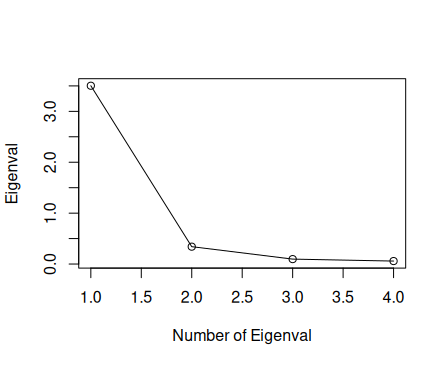
\includegraphics[scale=0.7]{./figures/scree_plot.png}
      \end{center}
      \par\bigskip
    \item There are numerous methods to decide how many components to include in the study. We can use the elbow-method in the scree plot or we can use the explained variance proportion which is given by:
      \begin{equation*}
        \begin{gathered}
          \dfrac{\sum_{j=1}^{k}\lambda_j}{\sum_{i=1}^{n}\lambda_i} = \text{ variance explained by the $k$th eigenvalues }
        \end{gathered}
      \end{equation*}
      \par\bigskip
      \noindent Personally I would have used 2 components, since this seems to be the elbow in the scree plot. Computing the variance explained yields:
      \begin{equation*}
        \begin{gathered}
          \dfrac{3.50293864+0.34142136}{3.50293864+0.34142136+0.09706136+0.05857864} \approx 96\%\text{ explained}
        \end{gathered}
      \end{equation*}
  \end{enumerate}
\end{enumerate}
